\documentclass[11pt]{article}

% ====================================================
% PACKAGES
% ====================================================
\usepackage[margin=1in, headheight=13.6pt]{geometry}
\usepackage[T1]{fontenc}
\usepackage{lmodern}
\usepackage{microtype}
\usepackage{setspace}
\usepackage{tcolorbox}
\usepackage{amsmath, amssymb, mathtools}
\usepackage{siunitx}
\usepackage{bm}

\usepackage{graphicx}
\usepackage{float}
\usepackage{subcaption}

\usepackage{enumitem}
\usepackage{booktabs}
\usepackage{longtable}
\usepackage{array}
\usepackage{multirow}

\usepackage{xcolor}
\usepackage{hyperref}

\usepackage{fancyhdr}
\usepackage{lastpage}

\usepackage{indentfirst}
\usepackage[justification=centering]{caption}
\usepackage{pdfpages}
\usepackage{listings}

\lstdefinestyle{pystyle}{
    language=Python,
    basicstyle=\ttfamily\small,
    keywordstyle=\color{blue!60!black}\bfseries,
    commentstyle=\color{green!40!black}\itshape,
    stringstyle=\color{orange!70!black},
    numbers=left,
    numberstyle=\tiny\color{gray},
    numbersep=6pt,
    breaklines=true,
    breakatwhitespace=false,
    showstringspaces=false,
    frame=single,
    rulecolor=\color{gray!50},
    tabsize=4
}
\lstset{style=pystyle}

\pagestyle{fancy}
\fancyhf{}
\lhead{\Assignment\ |\ \course}
\rhead{\Name\ |\ \today}
\cfoot{Page \thepage\ of~\pageref{LastPage}}

\hypersetup{
    colorlinks,
    linkcolor={red!50!black},
    citecolor={blue!50!black},
    urlcolor={blue!80!black}
}

\newcommand{\Name}{Arael Anaya}
\newcommand{\Assignment}{Homework 8}
\newcommand{\course}{Robot Mechanics}

% Boxed final-answer environment
\newtcolorbox{result}{
    colback=blue!3!white,
    colframe=blue!40!black,
    boxrule=0.6pt,
    arc=2pt,
    left=6pt, right=6pt, top=4pt, bottom=4pt
}

% Boxed problem-statement environment
\newtcolorbox{statement}{
    colback=gray!5!white,
    colframe=gray!50!black,
    boxrule=0.4pt,
    arc=2pt,
    left=6pt, right=6pt, top=4pt, bottom=4pt
}

% Visible placeholder for work not yet added
\newcommand{\workplaceholder}{%
    \par\vspace{4pt}\noindent\textcolor{gray!60}{\itshape [Work not yet added: paste solution here]}\par\vspace{4pt}%
}

% Boxed correction-note environment (flags a fix made to the original hand calc)
\newtcolorbox{fixnote}{
    colback=orange!5!white,
    colframe=orange!55!black,
    boxrule=0.5pt,
    arc=2pt,
    left=6pt, right=6pt, top=4pt, bottom=4pt,
    fontupper=\small
}

% Notation macros (matching course conventions)
\newcommand{\T}{\bm{T}}
\newcommand{\R}{\bm{R}}
\newcommand{\dvec}{\bm{d}}
\newcommand{\framen}[1]{\{#1\}}
\newcommand{\khat}{\widehat{\bm{k}}}
\newcommand{\wvec}{\bm{\omega}}
\newcommand{\xivec}{\bm{\xi}}
\newcommand{\vvec}{\bm{v}}
\newcommand{\Omvec}{\bm{\Omega}}
\newcommand{\Rotx}{\operatorname{Rot}_x}
\newcommand{\Roty}{\operatorname{Rot}_y}
\newcommand{\Rotz}{\operatorname{Rot}_z}
\newcommand{\atantwo}{\operatorname{atan2}}
\newcommand{\skewx}[1]{\left[#1\right]_{\times}}

\begin{document}

% ====================================================
% PROBLEM 1
% ====================================================
\section*{Problem 1}

\begin{statement}
Consider a three-link manipulator with the following DH table.
\begin{center}
\begin{tabular}{c|cccc}
Link & $a$ & $d$ & $\alpha$ & $\theta$  \\ \hline
1 & $0$ & $L_1$ & $\pi/2$ & $\star$ \\
2 & $L_2$ & $0$ & $0$ & $\star$ \\
3 & $L_3$ & $0$ & $0$ & $\star$
\end{tabular}
\end{center}
\begin{enumerate}[label=(\alph*), nosep]
\item Derive the forward kinematic equations symbolically for the position of the end effector in the base frame as a function of $\theta_1$, $\theta_2$, and $\theta_3$.
\item Symbolically differentiate these kinematic equations to construct a symbolic representation of the position rows of the velocity Jacobian.
\item Using the method outlined in class, calculate ${}^0\bm{z}_{k-1}$ and ${}^0\dvec_{k-1,N}$ for all $k=1,\ldots,N$ symbolically and construct the position rows of the velocity Jacobian.
\item For $L_1=1$\,m, $L_2=0.5$\,m, $L_3=0.3$\,m, $\theta_1=0$\,rad, $\theta_2=\pi/4$\,rad, and $\theta_3=\pi/4$\,rad, numerically evaluate your results from (b) and (c). \emph{Hint: They should match!}
\end{enumerate}
\end{statement}

\textbf{Solution.} Abbreviations: $c_i=\cos\theta_i$, $s_i=\sin\theta_i$, $c_{23}=\cos(\theta_2+\theta_3)$, $s_{23}=\sin(\theta_2+\theta_3)$. With $\cos\frac{\pi}{2}=0$ and $\sin\frac{\pi}{2}=1$, the DH transform
\[
\bm{A}_i=\operatorname{Rot}_z(\theta_i)\operatorname{Trans}_z(d_i)\operatorname{Trans}_x(a_i)\operatorname{Rot}_x(\alpha_i)=
\begin{bmatrix}
c_{\theta}&-s_{\theta}c_{\alpha}&s_{\theta}s_{\alpha}&a\,c_{\theta}\\
s_{\theta}&c_{\theta}c_{\alpha}&-c_{\theta}s_{\alpha}&a\,s_{\theta}\\
0&s_{\alpha}&c_{\alpha}&d\\
0&0&0&1
\end{bmatrix}
\]
gives the link transforms
\[
{}^0\T_1=\begin{bmatrix}c_1&0&s_1&0\\s_1&0&-c_1&0\\0&1&0&L_1\\0&0&0&1\end{bmatrix},\quad
{}^1\T_2=\begin{bmatrix}c_2&-s_2&0&L_2c_2\\s_2&c_2&0&L_2s_2\\0&0&1&0\\0&0&0&1\end{bmatrix},\quad
{}^2\T_3=\begin{bmatrix}c_3&-s_3&0&L_3c_3\\s_3&c_3&0&L_3s_3\\0&0&1&0\\0&0&0&1\end{bmatrix}.
\]

\paragraph{(a) Forward kinematics.} Multiplying the first two links,
\[
{}^0\T_2=\begin{bmatrix}c_1c_2&-c_1s_2&s_1&L_2c_1c_2\\s_1c_2&-s_1s_2&-c_1&L_2s_1c_2\\s_2&c_2&0&L_1+L_2s_2\\0&0&0&1\end{bmatrix},
\]
and then ${}^0\T_3={}^0\T_1\,{}^1\T_2\,{}^2\T_3$ has the rotation block
\[
{}^0\R_3=\begin{bmatrix}c_1c_{23}&-c_1s_{23}&s_1\\s_1c_{23}&-s_1s_{23}&-c_1\\s_{23}&c_{23}&0\end{bmatrix},
\]
using $c_2c_3-s_2s_3=c_{23}$ and $c_2s_3+s_2c_3=s_{23}$. The end effector position is
\begin{result}
\[
{}^0\bm{p}={}^0\dvec_{0,3}=\begin{bmatrix}c_1\,(L_2c_2+L_3c_{23})\\ s_1\,(L_2c_2+L_3c_{23})\\ L_1+L_2s_2+L_3s_{23}\end{bmatrix}.
\]
\end{result}

\paragraph{(b) Differentiating the position.} The position rows of the Jacobian are $\bm{J}_v=\begin{bmatrix}\partial\bm{p}/\partial\theta_1&\partial\bm{p}/\partial\theta_2&\partial\bm{p}/\partial\theta_3\end{bmatrix}$:
\begin{result}
\[
\bm{J}_v=\begin{bmatrix}
-s_1\,(L_2c_2+L_3c_{23}) & -c_1\,(L_2s_2+L_3s_{23}) & -L_3\,c_1s_{23}\\
\phantom{-}c_1\,(L_2c_2+L_3c_{23}) & -s_1\,(L_2s_2+L_3s_{23}) & -L_3\,s_1s_{23}\\
0 & L_2c_2+L_3c_{23} & L_3\,c_{23}
\end{bmatrix}.
\]
\end{result}

\paragraph{(c) Geometric method.} All joints are revolute, so column $k$ is ${}^0\bm{z}_{k-1}\times{}^0\dvec_{k-1,3}$. The joint axes are the third columns of ${}^0\R_{k-1}$:
\[
{}^0\bm{z}_0=\begin{bmatrix}0\\0\\1\end{bmatrix},\qquad
{}^0\bm{z}_1={}^0\bm{z}_2=\begin{bmatrix}s_1\\-c_1\\0\end{bmatrix}.
\]
The vectors from each joint origin to the end effector are ${}^0\dvec_{k-1,3}={}^0\bm{p}_{0,3}-{}^0\bm{p}_{0,k-1}$. Subtracting $L_1$ from the $z$-entry of ${}^0\bm{p}$ gives $\dvec_{1,3}$, and subtracting the origin of frame 2 gives $\dvec_{2,3}$:
\[
{}^0\dvec_{0,3}=\begin{bmatrix}c_1(L_2c_2+L_3c_{23})\\ s_1(L_2c_2+L_3c_{23})\\ L_1+L_2s_2+L_3s_{23}\end{bmatrix},\quad
{}^0\dvec_{1,3}=\begin{bmatrix}c_1(L_2c_2+L_3c_{23})\\ s_1(L_2c_2+L_3c_{23})\\ L_2s_2+L_3s_{23}\end{bmatrix},\quad
{}^0\dvec_{2,3}=L_3\begin{bmatrix}c_1c_{23}\\ s_1c_{23}\\ s_{23}\end{bmatrix}.
\]
Taking the cross products column by column, with $\rho=L_2c_2+L_3c_{23}$ and $h=L_2s_2+L_3s_{23}$:
\[
\bm{z}_0\times\dvec_{0,3}=\begin{bmatrix}-s_1\rho\\c_1\rho\\0\end{bmatrix},\quad
\bm{z}_1\times\dvec_{1,3}=\begin{bmatrix}-c_1h\\-s_1h\\\rho\end{bmatrix},\quad
\bm{z}_2\times\dvec_{2,3}=L_3\begin{bmatrix}-c_1s_{23}\\-s_1s_{23}\\c_{23}\end{bmatrix}.
\]
Stacking these reproduces exactly the matrix found in (b).

\paragraph{(d) Numerical check.} For $L_1=1$\,m, $L_2=0.5$\,m, $L_3=0.3$\,m, $\theta_1=0$, $\theta_2=\theta_3=\pi/4$: $c_{23}=0$, $s_{23}=1$, $\rho=0.5\cos\frac{\pi}{4}=0.3536$, $h=0.5\sin\frac{\pi}{4}+0.3=0.6536$, and ${}^0\bm{p}=[0.3536,\ 0,\ 1.6536]^{\intercal}$\,m. Both methods (Appendix~A) give
\begin{result}
\[
\bm{J}_v^{(b)}=\bm{J}_v^{(c)}=\begin{bmatrix}
0&-0.6536&-0.3000\\
0.3536&0&0\\
0&0.3536&0
\end{bmatrix}\ \mathrm{m/rad},
\]
\end{result}
with a maximum entry-wise difference of $0$, so the two results match.

\bigskip
% ====================================================
% APPENDIX A: CODE
% ====================================================
\newpage
\section*{Appendix A: Code}

% Listings are skipped until the code file exists, so a missing file cannot break the build.
\newcommand{\codelisting}[2]{%
    \IfFileExists{../Code/#1}{\lstinputlisting[language=#2, caption={\detokenize{#1}}]{"../Code/#1"}}%
    {\noindent\textcolor{gray!60}{\itshape [#1 not yet written]}}%
}

\subsection*{Problem1.m}\codelisting{Problem1.m}{Matlab}

% ====================================================
% APPENDIX B: HAND CALCULATIONS
% ====================================================
\newpage
\section*{Appendix B: Hand Calculations}\label{app:hand}

\IfFileExists{../Homework_8_hand_calcs.png}{%
    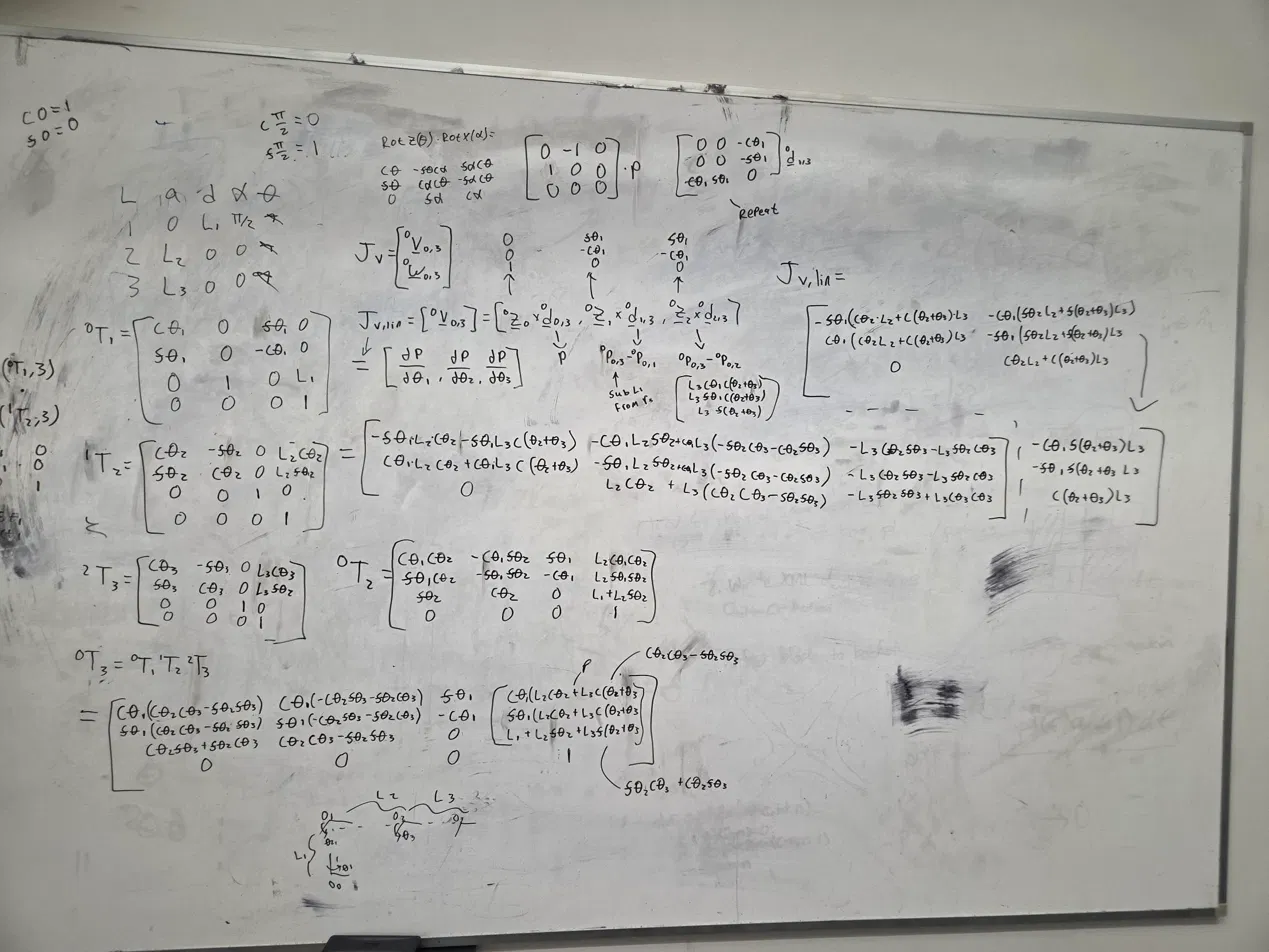
\includepdf[pages=-, landscape, pagecommand={\thispagestyle{plain}}, scale=0.95]{../Homework_8_hand_calcs.png}%
}{\noindent\textcolor{gray!60}{\itshape [Homework\_8\_hand\_calcs.png not yet added]}}

\end{document}
